\documentclass{article}

\usepackage[utf8]{inputenc}
\usepackage[margin=2cm]{geometry}
\usepackage{multicol}
\usepackage{float}
\usepackage{graphicx}
\graphicspath{{images/navigation/}{images/app/}{images/overview/}}

\title{Software Design Study Report}
\author{A-Team}

\begin{document}
\maketitle

%\begin{multicols}{2}
\begin{abstract}
Cars are ubiquitous in our modern lifestyles, unfortunately, the software systems in them do not keep up with other computing systems that we use. In this report, we aim to show how we tackled the problems and areas for improvement that we found in current car systems. Five areas of a modern car's feature set were focused on weekly, these being; the dashboard, media, navigation, safety and an accompanying smartphone app.
\end{abstract}

\section*{Introduction}
For years car companies have invested relatively little into their car's information systems and technological abilities. Inbuilt Sat Nav systems are often hard to use, update and are counter-intuitive. Since car companies are slow to adopt new technologies, even features that would have been possible many many years ago have not been widely used yet. For example, we still use the physical dials in the instrument cluster that we have used for years.

We have created an attractive and modern solution for digital technology in a car that we hope to see in future modern cars in production. In Section~\ref{sec:system-design} we will give explain the technical elements of our system design that can be found ranging from navigation to safety features. In Section~\ref{sec:nav} we will go into detail on the design process of our navigation system. In Section~\ref{sec:app} we will go into detail on the design process of our accompanying smartphone app.

\section{Overall system design}\label{sec:system-design}
\subsection{Algorithms}\label{ssec:algorithms}
\begin{itemize}
  \item Bidirectional A* Algorithm
    \begin{itemize}
      \item Heuristics
      % Talk about 
    \end{itemize}
  \item K means algorithm --- grouping convoys
  \item Learning algorithm --- user preferences, Contextually Aware Routing etc
    % FIND A LEARNING ALGORITHM
  \item Safety Detection algorithms
    \begin{itemize}
      \item Head pose algorithm
      \item Tesla radar system?
      \item Recognising bikes --- trained from training images which are bikes with riders
        % This is if we are detecting bikes using this method of detecting bikes (we mentioned using the 360 degree vision from the cameras for seeing bikes)
    \end{itemize}
  \item Something for tiredness detection
\end{itemize}

\subsection{Data Structures - Chris}\label{ssec:data-structures}
In the system that we have designed, we require a few different data structures in order make our system efficient and easy to work with.

For our navigation algorithm we decided to model the street map as a graph. Road junctions, route starting point and route destination are all represented as nodes in the graph, with roads being the edges that connect the nodes of the graph. This graph structure is most appropriate for us to use in our bidirectional A* search algorithm.

Routes will be kept in a JSON format with a JSON object containing two lists, one list containing nodes IDs of a route and the other containing the edge IDs. List items will be in chronological order for the route. The system is able to present the route on-screen by reading the lists to build the section of the street map graph that represents the route. This JSON format also allows for sections of the route to be updated easily by swapping out and adding nodes and edges. Another benefit of this format is that it is easy to implement the transferring of these routes from the app to the car.

The customisable dashboard layout will also be stored in a JSON format with widgets stored in a list object and more general details in a separate object. Widget objects in the list contain information about their relative position, size and styling in the dashboard.

User profile data such as username, route preferences etc.\ will all be kept in an encrypted Oracle database in the cloud, this will allow for us to have granular control over what information we receive when requesting user information.

An SQLite database will exist in the local storage of the car, this database will contain details of local music files that are also stored in the car's local storage. Music files that have been added to the car will have their song, album and artist names looked up and stored in the database. The SQLite database provides access to song details to the centre console and car app.

The smartphone app for the car system will use the same data structure for maps as the car uses. The smartphone app will also use an SQLite database to cache data from the cloud and car such as profile usernames, schedule data etc.\ This is to allow the app to still be functional while data is updating from permanent storage locations.

\subsection{Storage - Chris}\label{ssec:storage}
\begin{itemize}
  \item Cloud storage% - Oracle Database
    \begin{itemize}
      \item Updated from the car and app
      \item User Profiles
        % What is stored here, Car Loc, Settings, Routes (synced with phone), Privileges, seat preferences, driver stats
      \item Convoy Groups
        % Data on member locations, group messages, routes, route changes etc
      \item Software updates
    \end{itemize}
  \item Car SSD Storage
    \begin{itemize}
      \item Cached data from the cloud
      \item Cached data from applications such as Spotify
      \item Local music files
      \item Synchronised contacts from phone
      \item Dash cam footage
    \end{itemize}
\end{itemize}

\subsection{User Accounts - Matt}\label{ssec:user-accounts} 
Something that we found is lacking across intelligent car systems in the market is the use of portable user profiles. By this we mean profiles that can be used across several cars, applying user settings and preferences where applicable. 
There are several ways in which such data can be encapsulated and moved from car to car, including serving a database from a server to the car, transport via Bluetooth directly from a smartphone, use of NFC tags and many others.
\subsubsection{Storage and transport}
The method we found most suitable for doing this works by storing the data relative to each user profile online in an SQLite database and then serving it either directly to the car when a user logs in from in-car interfaces or to a smartphone application. Following this, the user is able to transfer the data to the car via Bluetooth with the press of a button. The data is cached on the phone and car, as applicable, to allow access even when internet access is limited or not available.   
\subsubsection{Cardinality of accounts, vehicles and shared data}
Each user will have one account that will be able to contain multiple car profiles. Car profiles can share generic information, such as preferences regarding routing, music, favourite temperatures, speed dial contacts, etcetera if the user specifies so. Information specific to the car make and model, such as steering rack height, seat adjustments, wing mirror adjustments shall stay bonded to each car profile.
\begin{figure}[H]
  \centering
  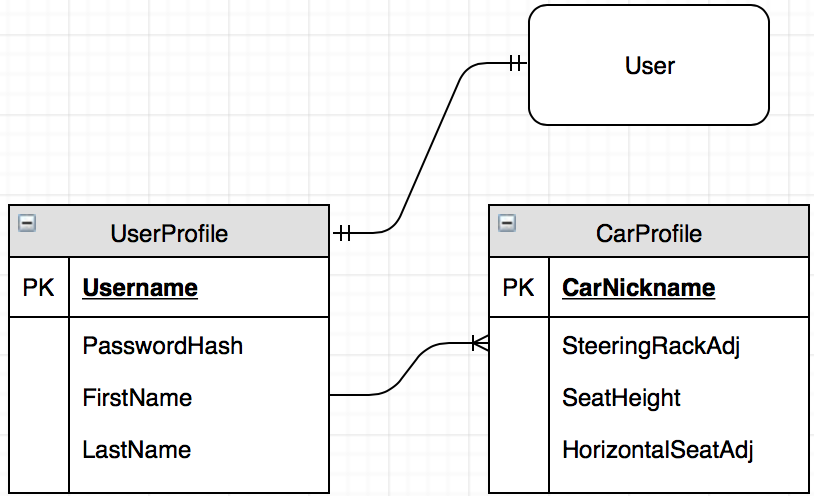
\includegraphics[scale=0.7]{profile-cardinality}
  \caption{Visualisation of cardinality of user profiles}\label{cardinality}
\end{figure}


\subsection{Communications \& Data Flows - Tyler}\label{ssec:communications-data}
Within our system, we have communications between the Mobile App, the Car and our Cloud, with links to external APIs.

\subsubsection{Communication between car and cloud}
\begin{itemize}
  \item Synchronisation with user profiles
  \item System updates
  \item Map updates
  \item Streaming camera feeds
  \item API calls to the cloud
  \item Real time event data, for example someone is breaking into your car, car stats (warning lights)
\end{itemize}
\subsubsection{Communication between car and phone}
Communications between the car and the phone consist of initial connection, instructions and data transfer. Establishing a connection is done by pairing the phone to the car by means of NFC, this will authenticate the phone with the car for communications over Bluetooth and Wi-Fi. Authentication can also be achieved by typical manual methods such as typing in a password. 
-- typical bluetooth things like sharing contacts/music over bluetooth/taking calls etc

Many features of the mobile app rely on communication with the car in order for them to work. These messages are sent between the phone to the car's central computing unit to be processed. Features which send instructions to the car to control the car's hardware have two different types of communication. 

Firstly, instructions such as turn the heating on or toggling headlights will be a be on an on/off basis. For example setting the temperature to 20 degrees will keep it at that until it has changed.

Secondly, instruction-critical tasks such as remote controlling the car with the phone app, rapidly send instructions to the car to ensure the car is performing actions safely and as the user expects. For example, if a user is holding the steering wheel at a 45 degree angle, the associated instruction will be sent constantly and processed by the central computing unit until the user changes the rotation. If the phone would happen to lose connection and the instructions stop being received by the car, the car is stopped.

Features for controlling music within the car are communicated over Wi-Fi and Bluetooth. The local music library of the car is synced with the phone, and also the spotify account linked to the drivers user profile is logged in on the centre console.

All messages regarding the control of music is encapsulated within a JSON object, this object will hol

-- Spotify: 
	-- Centre console can be controlled over wifi by multiple different user spotify accounts using SPOTIFY APP
    -- Done with spotify connect sdk
-- Our APP
	-- Local music synced with the car
		-- Our app shows the library of local music, which songs can be added/skipped etc
        -- Also have access to the spotify account on centre console for doing actions THROUGH that account

\begin{itemize}
  \item NFC pairing for Bluetooth and Wi-Fi
  \item Remote Control
  \item Media Control --- Song requests etc.
\end{itemize}
\subsubsection{Communication between phone and cloud}
\begin{itemize}
  \item Hashes and timestamps are compared on the server to decide what to synchronise
  \item API calls to the cloud
  \item Car camera feeds can be streamed to the phone on-demand over RTSP
  \item Information regarding convoy setup on phone
  \item Car software updates from cloud (Gives ability to update car with phone)
  \item Real time event data from cloud eg someone breaking into your car, car stats (warning lights)
\end{itemize}
\subsubsection{Communication between car and external APIs}
% Talk about how it connects to the cloud which provides a link to the APIs
\begin{itemize}
  \item Roadworks
  \item Traffic
  \item Weather
  \item Public Transport
  \item Note: All API calls are relative to the country the car is located in.
\end{itemize}

\begin{itemize}
  \item Communications between car and phone

  \item Communications between car and cloud (Over in-car LTE and external Wi-Fi if available)

  \item Communications between phone and cloud

  \item Communications between car and external APIs (API links and mappings provided from cloud)
\end{itemize}

\subsection{Information Security - Joe}\label{ssec:information-security}
A major focus for any internet connected technology is security, and with our car systems it is no different- the last thing a customer would want is to have their car stolen by it being driven into the distance by a remote thief. Security is a primary focus in every aspect of the car system, the following non-exhaustive list are some of our main focuses

\subsubsection{Data communication}
\subsubsection{Data storage \& encryption}
\subsubsection{User authentication}
\subsubsection{???}
\subsubsection{Profit}



\begin{itemize}
  \item Database encryption in the cloud
% * <frebib@gmail.com> 2017-03-20T22:31:12.891Z:
% 
% Is this a thing?
% Maybe the data can use end-to-end encryption, only unlockable with a key from the user account?
% ^ That however means the user is fleeced if they forget their password
% 
% ^.
  \item HTTPS for all internet communications
  \item WPA2-PSK with AES for Wi-Fi hotspot login
  \item X.509 certificate for the car
\end{itemize}

\subsection{Interaction Design - Matt}\label{sssec:interaction-design}
The interaction designs used on our product's interfaces were designed loosely based on designs from industry leading companies but tailored to integrate our ideas and implement some recurrent suggestions found throughout our research, which has seen over 100 responses. 
\subsubsection{Centre console}\label{1.7.1}
%%%%%%%%%%%%%%%%%%%%%
%	PLAN
%%%%%%%%%%%%%%%%%%%%%
\begin{itemize}
  \item Centre console
  \item Mobile phone
  \item Rear side door device
    % Justifications of why we have chosen these interfaces
\end{itemize}
\subsection{Aesthetics/Graphical Design - Matt}\label{ssec:aesthetics}
% User Interfaces of the above devices
An effort was made to follow current styling standards used in industry to give the user a familiar experience, therefore flat designs were used where possible. Also characterising our design are large icons and avoidance of large swathes of text.
\subsubsection{Dashboard cluster screen}\label{1.8.1}
A screen will be replacing the usual instrument cluster behind the steering wheel. This will display information relative to speed, engine revolutions, fuel levels as it has been doing for the past decades but with the twist

%%%%%%%%%%%%%%%%%%%%%
%	PLAN
%%%%%%%%%%%%%%%%%%%%%
\begin{itemize}
  \item Centre console
  \item Smaller navigation console above centre console
  \item Mobile phone
  \item Rear side door device
    % Justifications of why we have chosen these designs
\end{itemize}




%%%%%%%%%%%%%%
%
%	NAV
%
%%%%%%%%%%%%%%
\section{Feature 1: Navigation}\label{sec:nav}

\subsection{Research - Lewis}\label{ssec:nav-research}
\begin{itemize}
  \item Questionnaires
  \item Researching latest technology
\end{itemize}

\subsection{Brainstorming - Matt}\label{ssec:nav-brainstorming}
% Should we cite our initial ideas document?
Our first stage of brainstorming was to create a Google Drive document, in which we started writing down our ideas while discussing them and generating further ideas through our discussions. During this initial stage, all ideas discussed were noted down and not removed, to keep the design space open and to encourage further discussion of it in a later iteration. After this initial stage, and an iteration of research, we went through this document and discussed as a group what was worth expanding upon and taking forward to our final design.

An aid we found very useful was personas, a list of made-up personalities with realistic interests, jobs and attributes. During the brainstorming each of us tried to empathise with the different personas and think about their habits, things they enjoy, their mental states throughout different times of the day and from there, think of their needs, features they would enjoy and why.
\begin{itemize}
  \item Collectively worked together to put down all of our ideas into a google doc
  \item No ruling out of ideas
  \item Finally moved everything into a final document. Discussed each point as a group to decide what was worth expanding
  \item Things specific to the nav brainstorm i.e.\ the ideas to come out of it
\end{itemize}

\subsection{Tech background - Lewis}\label{ssec:nav-tech}
(Most of this seems like it would be algorithms again, so we plan to expand on the algorithms further than was detailed in section 2.1)
\begin{itemize}
  \item Bidirectional A* search
  \item K-means clustering
\end{itemize}

\subsection{Convoy - Chris}\label{ssec:nav-convoy}
\begin{itemize}
  \item Convoy interface
  \item Features
  \item App
\end{itemize}
% Include limitations of the above and how we combat them

\subsection{Design choices \& argumentation - Lewis}\label{ssec:nav-design}
\begin{itemize}
  \item QOC
  \item Justification for algorithms
    % Would this be better placed in the previous section?
    \begin{itemize}
      \item Routing
      \item Clustering
    \end{itemize}
\end{itemize}

\subsection{Prototypes \& user testing - Matt}\label{ssec:nav-prototypes-testing}
\begin{itemize}
  \item Lo-Fi and Hi-Fi prototypes of Navigation
\end{itemize}

\subsection{Final design}\label{ssec:nav-final-design}

\subsection{Evaluation \& how it fits into whole system}\label{ssec:nav-evaluation}




%%%%%%%%%%%%%%
%
%	APP
%
%%%%%%%%%%%%%%
\section{Feature 2: App}\label{sec:app}

\subsection{Research - Matt}\label{ssec:app-research}
Research and brainstorming were conducted in a cyclic manner to ensure that the latest technologies relevant to this sector of the automotive industry were taken into consideration. Extensive research revealed that most leading companies such as Jaguar, BMW and Tesla already offer multi-platform mobile apps that compliment their automobiles. Each of the above boasts at least one of the features that we intended to integrate into our systems such as remote control and seamless route porting from smartphone to car. From brainstorming through to coding the prototype, our focus was directed on how to improve on existing products and also integrate our novel features.
The research methods we used included a questionnaire, installing and using manufacturers apps on our mobile devices, browsing their websites and reading through papers and articles found through numerous searches on search engines.
\begin{itemize}
  \item Existing apps that accompany a car
  \item Current technology
  \item How personas might want to interact with an app
    % Link to a persona document in the appendix
\end{itemize}
\subsection{Brainstorming - Chris}\label{ssec:app-brainstorming}

\begin{itemize}
  % First 3 points are same as section 3.2
  \item Collectively worked together to put down all of our ideas into a Google doc
  \item No ruling out of ideas
  \item Finally moved everything into a final document. Discussed each point as a group to decide what was worth expanding
  \item Things specific to the app brainstorm i.e.\ the ideas to come out of it
\end{itemize}
\subsection{Tech background - Tyler}\label{ssec:app-tech}
\begin{itemize}
  \item Communication
    \begin{itemize}
      \item (See section 2.4?)
      \item To and from car
        \begin{itemize}
          \item Initial connection with the car (Bluetooth/Wi-Fi/RFID)
          \item Communicating remote control instructions
          \item Other instructions (Media control, Controlling hardware)
        \end{itemize}
      \item To and from Cloud
        \begin{itemize}
          \item Authenticating User profiles
          \item Syncing data
          \item Feeds which are streamed (Camera feeds)
          \item Information such as Car location
        \end{itemize}
    \end{itemize}
\end{itemize}
% Repeating what is said in communication (2.4) ^^

\subsection{Design choices \& argumentation - Lewis (maybe)}\label{ssec:app-design}
\begin{itemize}
  \item QOC (to be made)
\end{itemize}

\subsection{Prototypes \& user testing}\label{ssec:app-prototypes-testing}
\begin{figure}[H]
  \centering
  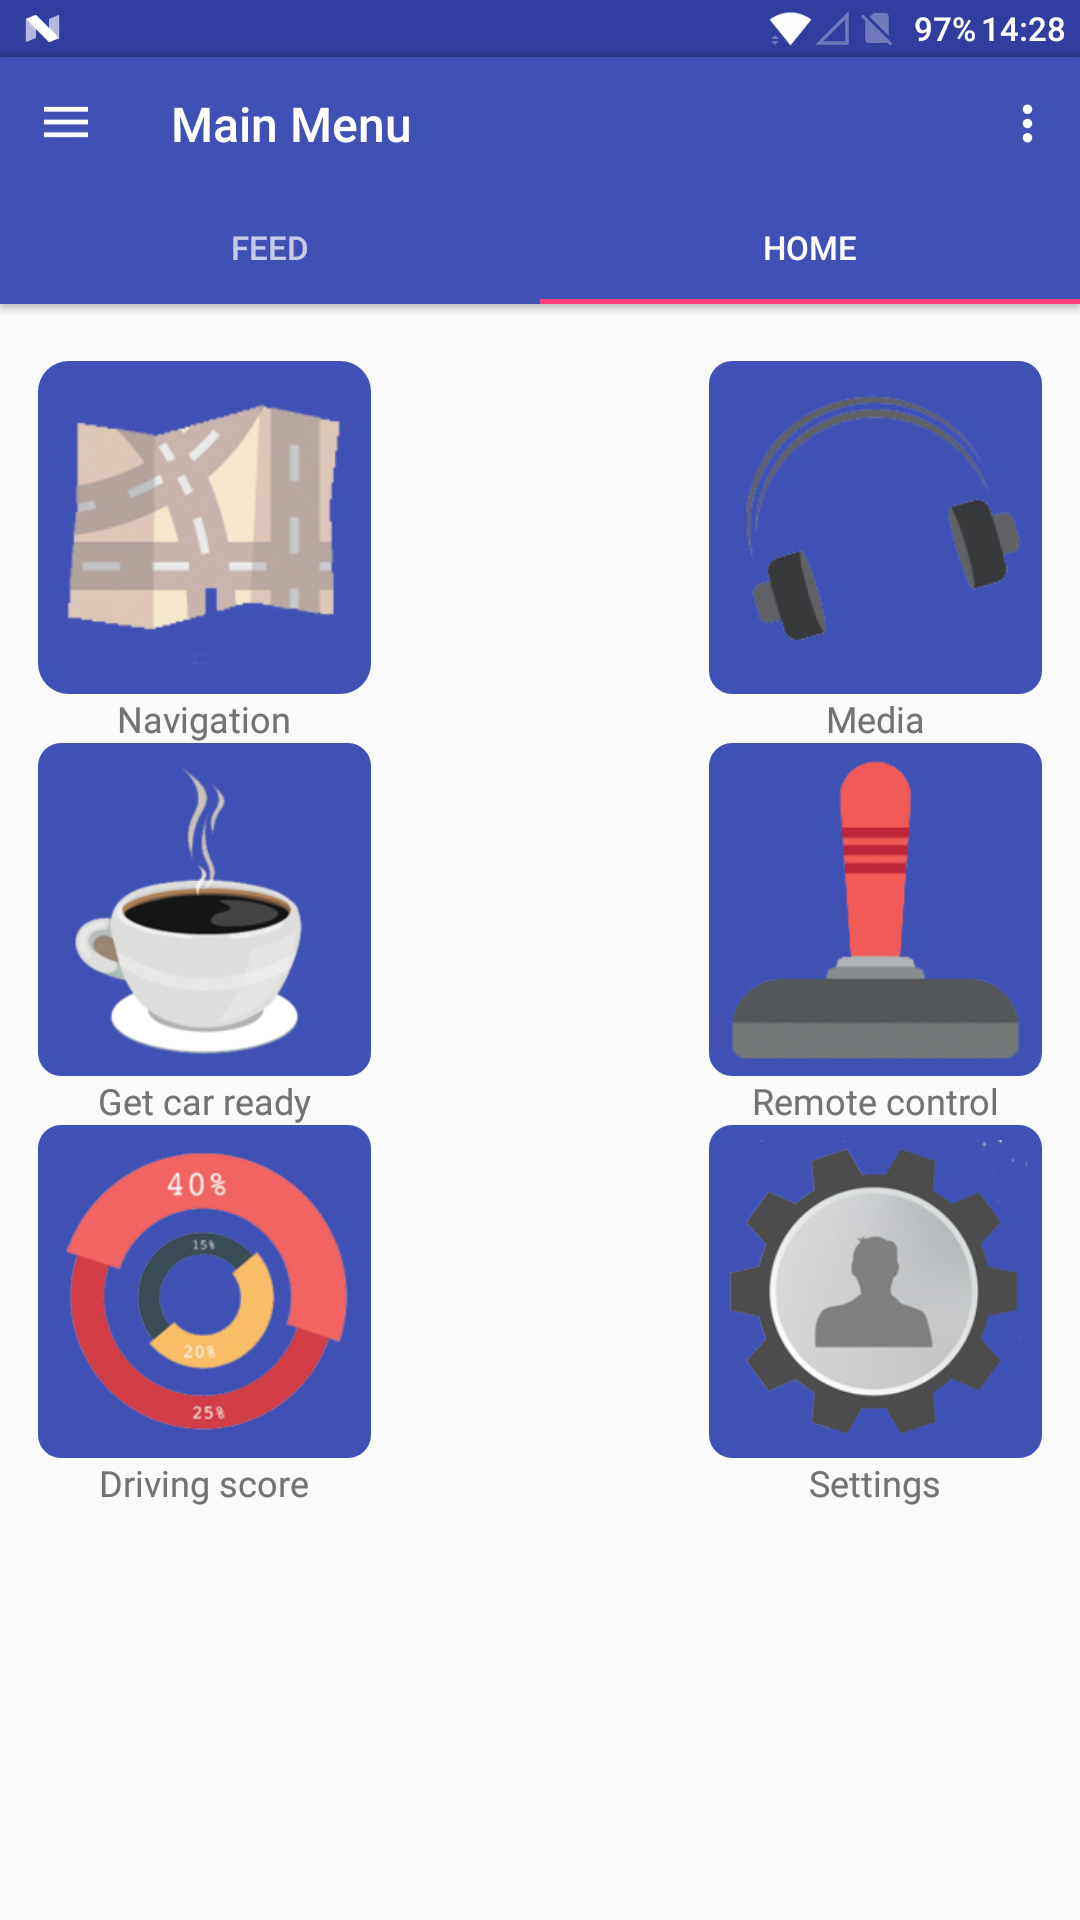
\includegraphics[scale=0.25]{main-menu}
  \caption{Hi-Fi prototype of app main menu.}\label{main-menu}
\end{figure}

\subsection{Final design}\label{ssec:app-final-design}

\subsection{Evaluation \& how it fits into whole system}\label{ssec:app-evaluation}

\section{Other areas}\label{sec:other}

Annotate slides on changes we would make going forwards
\section{References}\label{sec:references}

%\end{multicols}

\end{document}

% vim: set tabstop=2 shiftwidth=2:
